%%%%%%%%%%%%%%%%%%%%%%%%%%%%%%%%%%%%%%%%%
% Compact Academic CV
% LaTeX Template
% Version 1.0 (10/6/2012)
%
% This template has been downloaded from:
% http://www.LaTeXTemplates.com
%
% Original author:
% Dario Taraborelli (http://nitens.org/taraborelli/home)
%
% License:
% CC BY-NC-SA 3.0 (http://creativecommons.org/licenses/by-nc-sa/3.0/)
%
% Important:
% This template needs to be compiled using XeLaTeX
%
% Note: this template has the option to use the Hoefler Text font, see the
% font configurations section below for instructions on using this font
%
%%%%%%%%%%%%%%%%%%%%%%%%%%%%%%%%%%%%%%%%%

%----------------------------------------------------------------------------------------
%	PACKAGES AND OTHER DOCUMENT CONFIGURATIONS
%----------------------------------------------------------------------------------------

\documentclass[11pt, a4paper]{article} % Document font size and paper size

\usepackage{fontspec} % Allows the use of OpenType fonts

\usepackage{geometry} % Allows the configuration of document margins
%\geometry{a4paper,  textwidth=6in, textheight=9.7in, marginparsep=7pt, marginparwidth=0.5in} % Document margin settings
\geometry{a4paper, left=4cm, right=2.5cm, top=1.2in, bottom=1in, marginparwidth=1.5cm, marginparsep=7pt}
\setlength\parindent{0cm} % Remove paragraph indentation

\usepackage[usenames,dvipsnames]{xcolor} % Custom colors

\usepackage{sectsty} % Allows changing the font options for sections in a document
\usepackage[normalem]{ulem} % Custom underlining
\usepackage{xunicode} % Allows generation of unicode characters from accented glyphs
\defaultfontfeatures{Mapping=tex-text} % Converts LaTeX specials (``quotes'' --- dashes etc.) to unicode

\usepackage{marginnote} % For margin years
\newcommand{\years}[1]{\marginnote{\scriptsize #1}} % New command for including margin years
\renewcommand*{\raggedleftmarginnote}{}
\setlength{\marginparsep}{8pt} % Slightly increase the distance of the margin years from the contant
\reversemarginpar

\usepackage[xetex, bookmarks, colorlinks, breaklinks, pdftitle={Taihong Xiao - resume},pdfauthor={Taihong Xiao}]{hyperref} % PDF setup - set your name and the title of the document to be incorporated into the final PDF file meta-information
\hypersetup{linkcolor=blue,citecolor=blue,filecolor=black,urlcolor=MidnightBlue} % Link colors

\usepackage{amssymb}

\usepackage[final]{pdfpages}

%----------------------------------------------------------------------------------------
%	FONT CONFIGURATIONS
%----------------------------------------------------------------------------------------

% Two font choices are available in this template, the default is Linux Libertine, available for free at: http://www.linuxlibertine.org while the secondary choice is Hoefler Text which comes bundled with Mac OSX.
% To use Hoefler Text, comment out the Linux Libertine block below and uncomment the Hoefler Text block. You will also need to replace the "\&" characters with "\amper{}" in section titles.

%% Linux Libertine Font (default)
 \setromanfont[Ligatures={Common}, Numbers={OldStyle}, Variant=01]{Times New Roman}%{Linux Libertine O} % Main text font
%\setmonofont[Scale=0.8]{Monaco} % Set mono font (e.g. phone numbers)
\sectionfont{\mdseries\upshape\Large\bf} % Set font options for sections
\subsectionfont{\mdseries\scshape\normalsize} % Set font options for subsections
\subsubsectionfont{\mdseries\upshape\large} % Set font options for subsubsections
\chardef\&="E050 % Custom ampersand character

% Hoefler Text Font (bundled with Mac OSX)
%\setromanfont [Ligatures={Common}, Numbers={OldStyle}]{Hoefler Text} % Main text font
%\setmonofont[Scale=0.8]{Monaco} % Set mono font (e.g. phone numbers)
%\setsansfont[Scale=0.9]{Optima Regular} % Set sans font, used in the main name and titles in the document
%\newcommand{\amper}{{\fontspec[Scale=.95]{Hoefler Text}\selectfont\itshape\&}} % Custom ampersand character
%\sectionfont{\sffamily\mdseries\large\underline} % Set font options for sections
%\subsectionfont{\rmfamily\mdseries\scshape\normalsize} % Set font options for subsections
%\subsubsectionfont{\rmfamily\bfseries\upshape\normalsize} % Set font options for subsubsections

%----------------------------------------------------------------------------------------

\usepackage{float,graphicx,wrapfig,picins}
\usepackage{amsmath,mathrsfs}

% \usepackage{ccmap}

\usepackage{paralist}

\setlength{\itemsep}{2pt}
\newcommand{\alert}[1]{\textcolor{red}{\bf #1}}

\linespread{1.1}


% head 
%\usepackage{fancyhdr}
%
%\pagestyle{fancy}
%\fancyhf{}
%\fancyhead[L]{%
%%  Taihong Xiao\ %(\href{mailto:xiaotaihong@pku.edu.cn}{\textcolor{blue}{\tt xiaotaihong@pku.edu.cn}})
%Resume (U-M ID: 48306744)
%  \rhead{Computer Science and Engineering (PhD) Fall 2018}
%}
%\cfoot{\thepage}

\begin{document}

%----------------------------------------------------------------------------------------
%	CONTACT AND GENERAL INFORMATION SECTION
%----------------------------------------------------------------------------------------
\parpic[r]{
\includegraphics[width=2.5cm]{pku_logo}}
%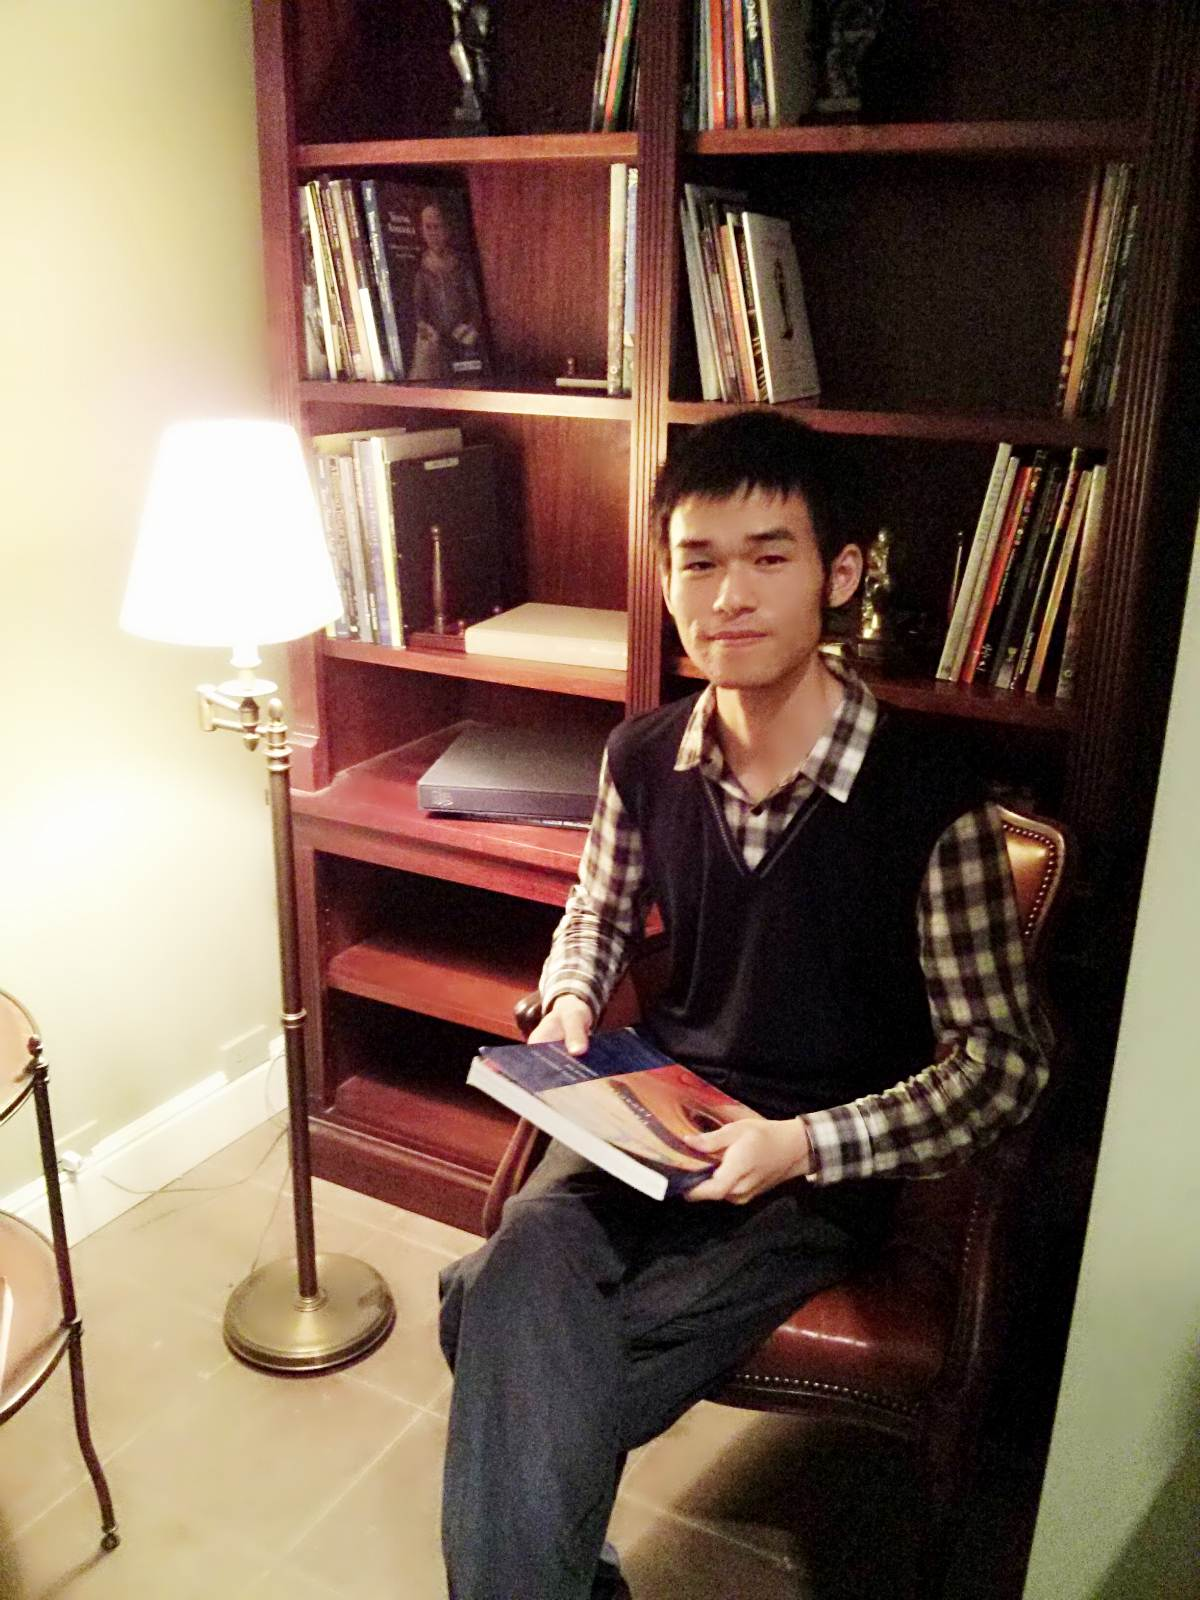
\includegraphics[width=3.5cm]{Profile.jpg}

%\begin{wrapfigure}{r}{0.3\textwidth}
%    \centering
%    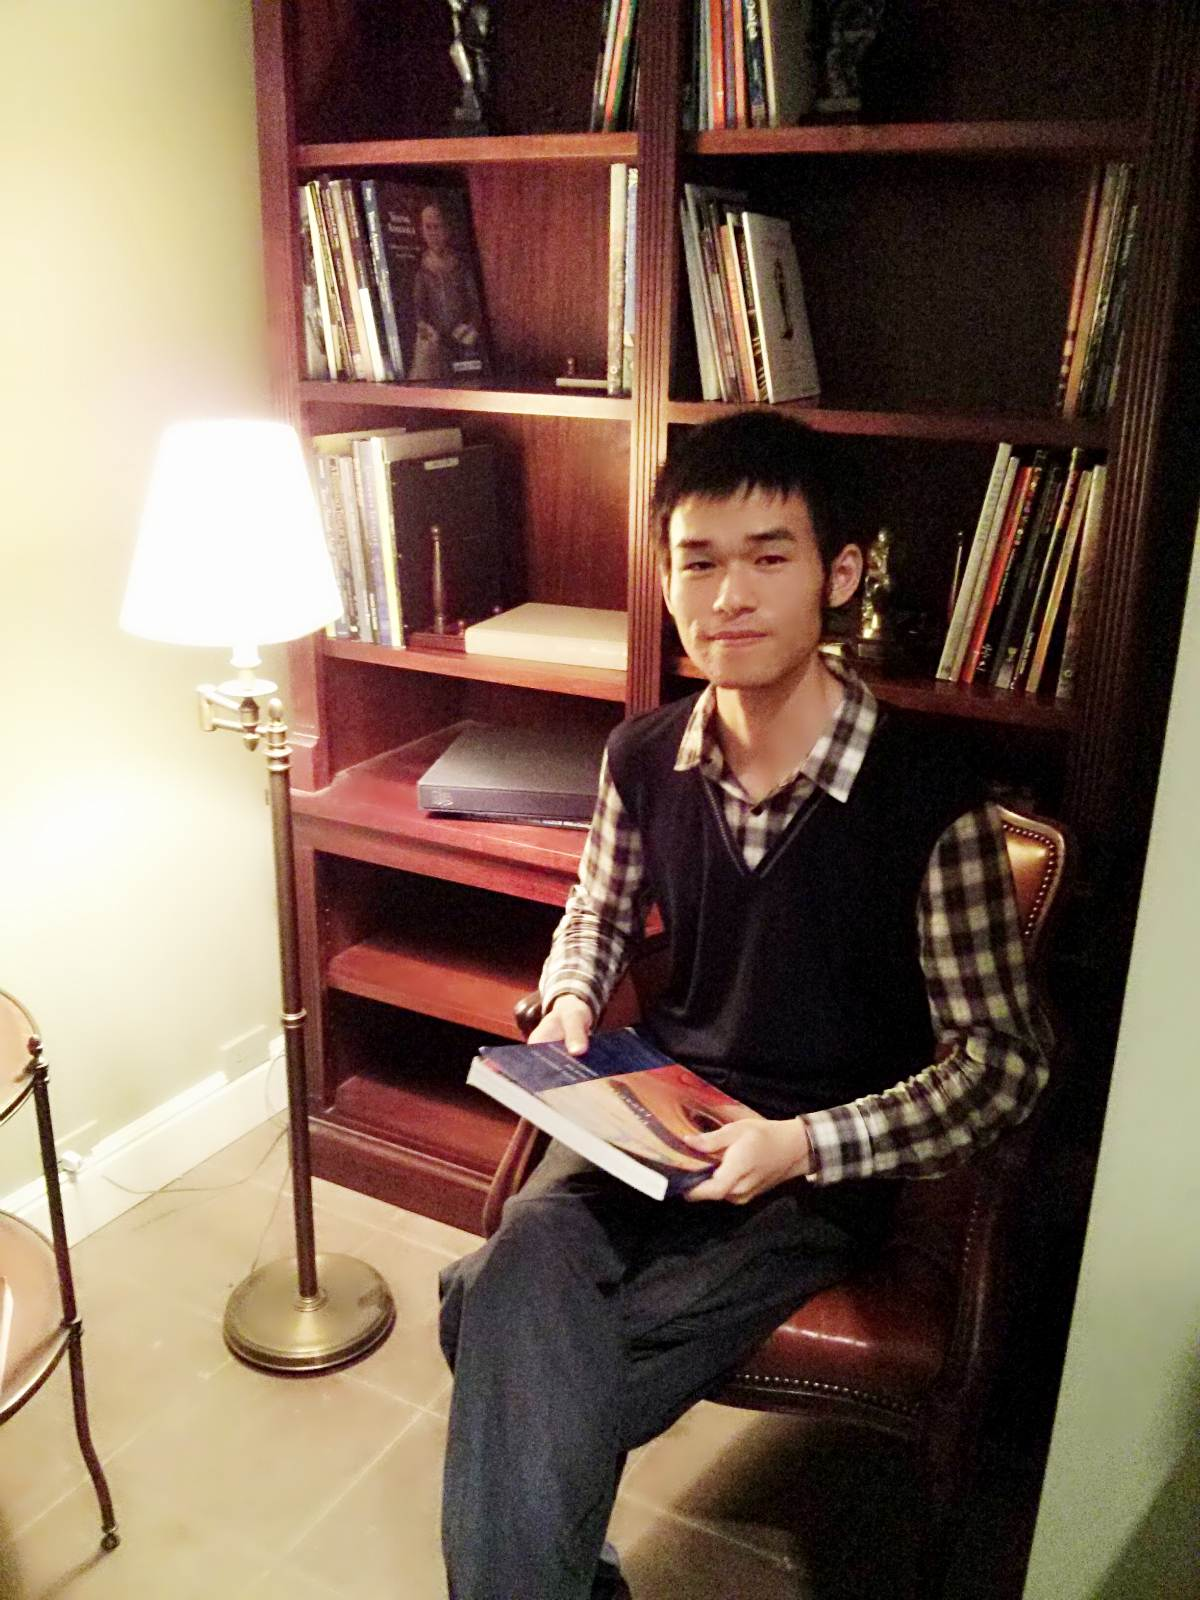
\includegraphics[width=3.5cm]{Profile.jpg}
%\end{wrapfigure}

{\LARGE\bf Taihong Xiao}\\[0.cm] % Your name

%\begin{float}
%\begin{minipage}
%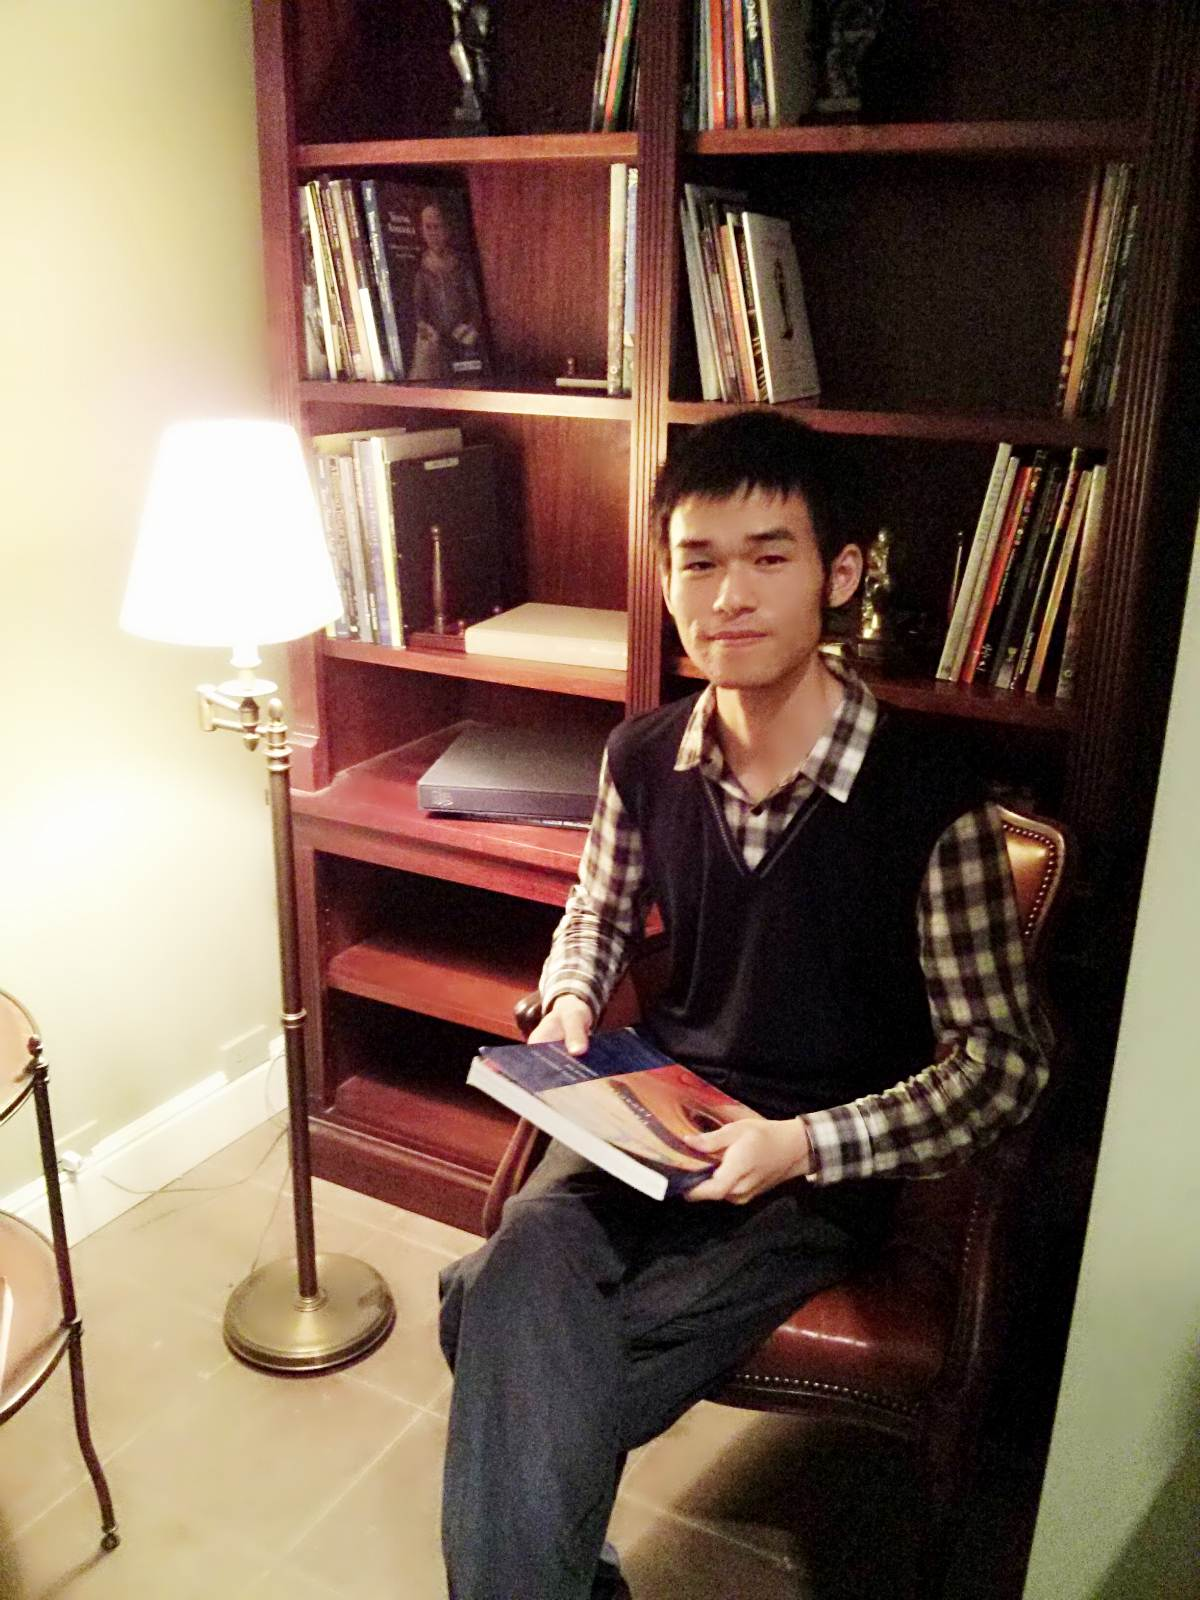
\includegraphics[width=0.3\linewidth]{Profile.jpg}
%\end{minipage}
%\end{float}

%\begin{wrapfigure}[2]{r}{0pt}
%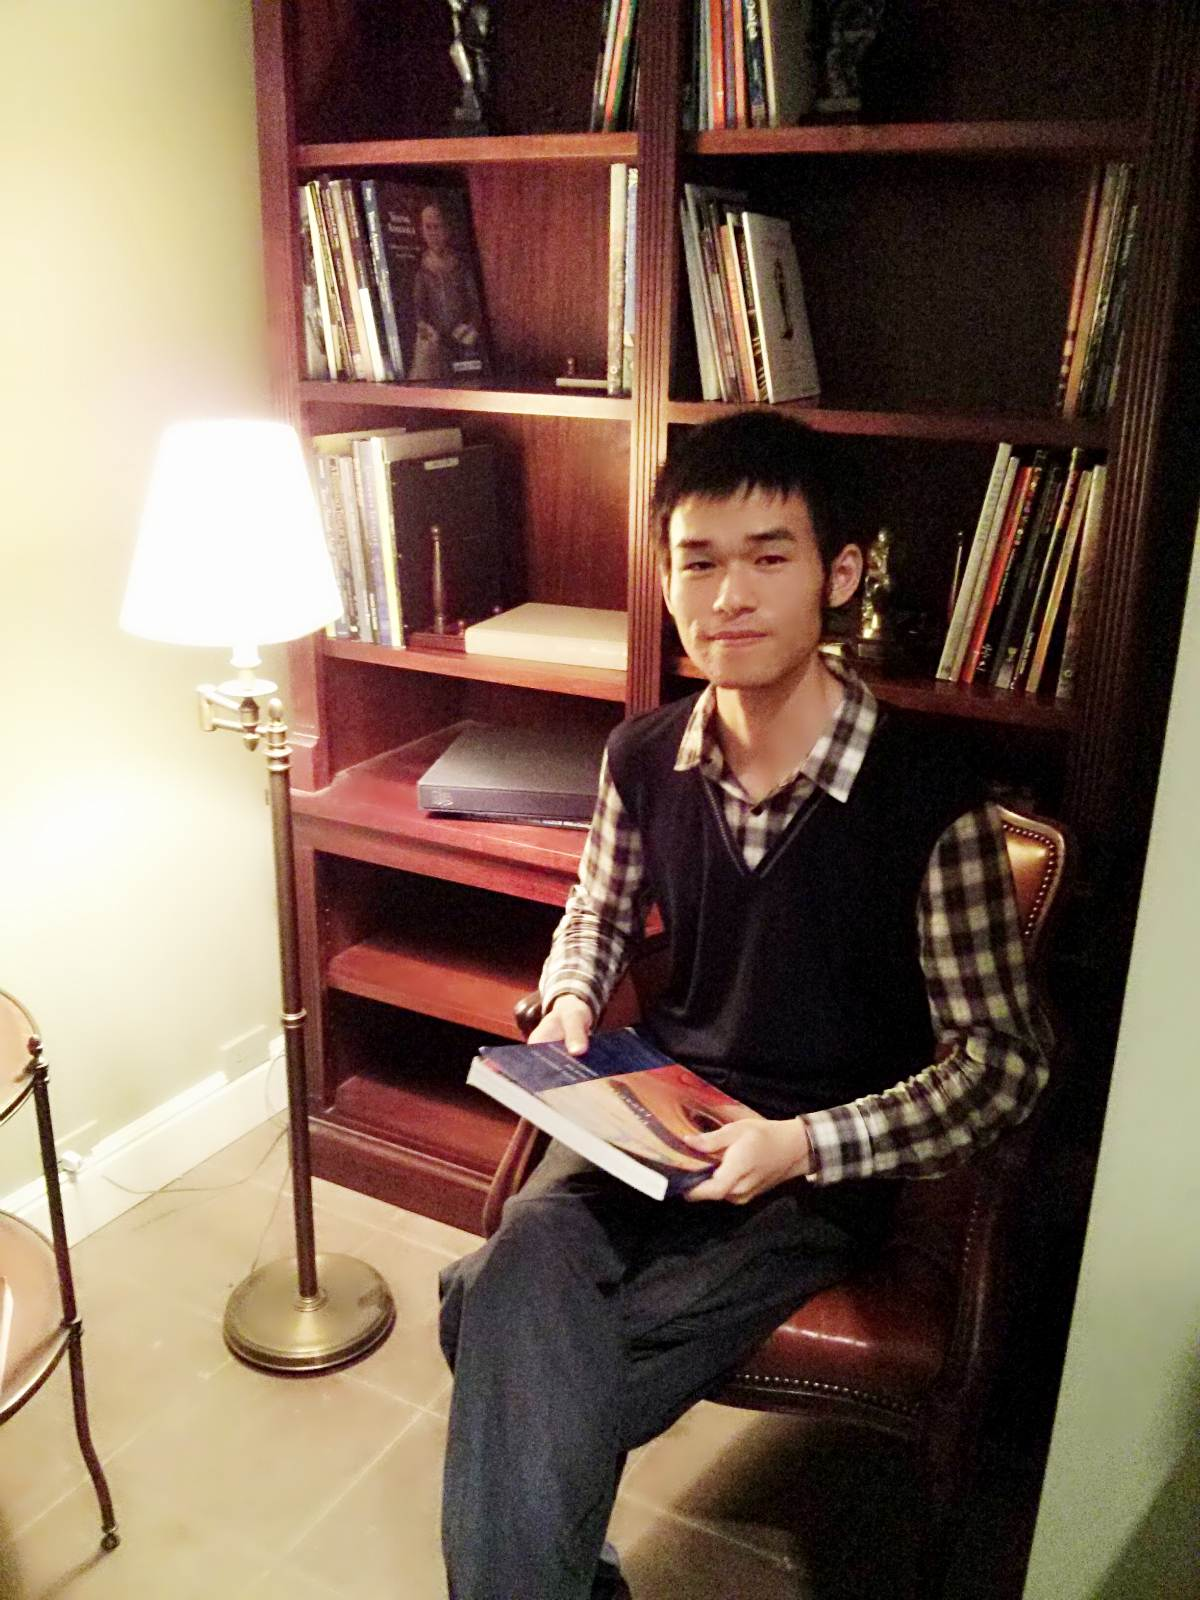
\includegraphics[width=0.2\textwidth]{Profile.jpg}
%\end{wrapfigure}



%\section*{Personal Information}

\years{Address} Peking University, Haidian District, Beijing, China, \texttt{100871} 

\years{Phone} \texttt{(86)18210929266}
% Fax: \texttt{609-924-8399}\\[.2cm] % Your fax number

\years{Email} \href{mailto:xiaotaihong@pku.edu.cn}{\tt xiaotaihong@pku.edu.cn}\quad
 \href{mailto:xiaotaihong@126.com}{\tt xiaotaihong@126.com}

\years{Homepage} \url{https://prinsphield.github.io} % Your academic/personal website

\years{GitHub} \url{https://github.com/Prinsphield}

\years{Research\\Interests} Computer Vision, Deep Learning, Machine Learning and Numerical Optimization


%----------------------------------------------------------------------------------------
%	EDUCATION SECTION
%----------------------------------------------------------------------------------------

\section*{Educations}

\years{2015.09-\\2018.07}\textbf{Department of Information Sciences, School of Mathematical Sciences, Peking University}

M.S. in Computer Vision, Deep Learning, Machine Learning\hfill GPA: 90/100, Rank: 1/34


\years{2013.06-\\2013.08}\textbf{Department of Mathematics, University of California, Berkeley}

Summer Session C. \hfill GPA: 3.6/4.0


\years{2011.09-\\2015.07}\textbf{Taishan College, Shandong University}

B.S. in Mathematics and Applied Mathematics. \hfill GPA: 88.02/100, Rank: 4/14


%----------------------------------------------------------------------------------------
%	RESEARCH INTERESTS SECTION
%----------------------------------------------------------------------------------------

%\section*{Research Interests}
%
%\years{} Machine Learning, Deep Learning, Computer Vision


%----------------------------------------------------------------------------------------
%	PUBLICATIONS SECTION
%----------------------------------------------------------------------------------------

\section*{Publications and Patents}

\years{2018}\textbf{ELEGANT: Exchanging Latent Encodings with GAN for Transferring Multiple Face Attributes}

Taihong Xiao, Jiapeng Hong and Jinwen Ma

\emph{European Conference on Computer Vision} \textbf{(ECCV)}, submitted

\href{https://arxiv.org/abs/1803.10562}{[ArXiv]}
\href{https://github.com/Prinsphield/ELEGANT}{[GitHub]}


\years{2018}\textbf{DNA-GAN: Learning Disentangled Representations from Multi-Attribute Images}

Taihong Xiao, Jiapeng Hong and Jinwen Ma

\emph{International Conference on Learning Representations} \textbf{(ICLR)}, Workshop Track

\href{https://openreview.net/pdf?id=rkX1FF_UM}{[OpenReview]} 
\href{https://arxiv.org/abs/1711.05415v2}{[ArXiv]}
\href{https://github.com/Prinsphield/DNA-GAN}{[GitHub]}
\href{https://prinsphield.github.io/ICLR-2018/poster/poster.pdf}{[Poster]}


%\years{2017}\textbf{Low-Rank Tensor Decomposition Using $\ell_p$-norm Optimization on the Matrix Manifold}
%
%Taihong Xiao and Jinwen Ma
%
%\emph{Journal of Computational and Applied Mathematics}, Under review

\years{2017}\textbf{GeneGAN: Learning Object Transfiguration and Attribute Subspace from Unpaired Data}

Shuchang Zhou, Taihong Xiao, Yi Yang, Dieqiao Feng, Qinyao He and Weiran He

\emph{British Machine Vision Conference} \textbf{(BMVC)}, \textbf{Oral} 

\href{http://arxiv.org/abs/1705.04932}{[ArXiv]}
\href{http://zsc.github.io/GeneGAN-BMVC2017.pdf}{[Slide]}
\href{https://github.com/Prinsphield/GeneGAN}{[GitHub]}


\years{2017}\textbf{IQNN: Training Quantized Neural Networks with Iterative Optimizations}

Shuchang Zhou, He Wen, Taihong Xiao and Xinyu Zhou

\emph{International Conference on Artificial Neural Networks} \textbf{(ICANN)}

\href{https://link.springer.com/chapter/10.1007\%2F978-3-319-68612-7_78}{[Paper]} 

\years{2017}\textbf{An Integrated Learning Framework for Pedestrian Tracking}

Taihong Xiao and Jinwen Ma

\emph{International Conference on Intelligent Computing} \textbf{(ICIC)}, \textbf{Oral}

\href{https://link.springer.com/chapter/10.1007\%2F978-3-319-63315-2_9}{[Paper]}
\href{https://prinsphield.github.io/extra/ICIC-20170808.pdf
}{[Slide]}
\href{https://github.com/Prinsphield/ILFPT}{[GitHub]}
\href{https://youtu.be/HQIi0Z9b4Pw}{[Video]}

\years{2017.09\\CN Patent}\textbf{A Head-detection Based Face Tracking Method}

Taihong Xiao, Shuchang Zhou and Yuchao Pan

\emph{Chinese Patent}, CN201710253546.5, In Process

%----------------------------------------------------------------------------------------
%	RESEARCH & WORKING EXPERIENCES SECTION
%----------------------------------------------------------------------------------------

\section*{Research Experience}

\years{2017.01-\\2017.11}{\bf Research Intern. Megvii (Face++) Inc. Beijing}\hfill 
\mbox{Advisor: Dr.~\href{https://zsc.github.io/}{Shuchang Zhou}}

{\bf $\blacktriangleright$ Face Attributes Transfiguration}\quad I  proposed a cross-domain image translation method named GeneGAN to achieve generate multi-modal images of a certain attribute. I participated most of experiments using our proprietary MegDL framework, and reproduce them using TensorFlow. This paper was published in BMVC 2017 for an oral presentation.

{\bf $\blacktriangleright$ Quantized Neural Networks}\quad I participated the research of compressing and accelerating neural networks. We proposed an multi-bit quantization algorithm that iteratively  solves for optimal scaling factor to reduce quantization errors. Besides, I did experiments of iterative training using TensorFlow. This paper was published in ICANN 2017.

\years{2016.01-\\present}{\bf Research Assistant. School of Mathematical Sciences and Key Laboratory of Mathematics and Its Applications, Peking University.} \hfill
\mbox{Advisor: Prof.~\href{http://www.math.pku.edu.cn/is/~jwma/}{Jinwen Ma}}

{\bf $\blacktriangleright$ Multiple Face Attribute Transfer.}\quad I proposed the ELEGANT model for transferring multiple face attributes. The model overcomes three limitations existing in many other methods: 1) failing to do image generation by exemplars; 2) unable to deal with multiple face attributes simultaneously; 3) bad quality of generated images, such as images of low-resolution or with lots of artifacts.

{\bf $\blacktriangleright$ Disentangled Representations}\quad I proposed DNA-GAN for learning disentangled representations from multi-attribute images. The annihilating operation could prevent from trivial solutions and the iterative training strategy overcame the difficulty of training on unbalanced datasets. This paper was accepted to ICLR 2018 workshop track.

{\bf $\blacktriangleright$ Tensor Decomposition}\quad I proposed a low-rank tensor decomposition method via $\ell_p$-norm optimization on matrix manifolds. Theoretically, I proved that the optimal solution to our $\ell_p$-norm variational form is equivalent to the matrix SVD in the two-way case, and the tensor SVD if the tensor is orthogonally decomposable in the higher-order case. This paper was under review at JCAM.

{\bf $\blacktriangleright$ Pedestrian Tracking}\quad I proposed an integrated framework for pedestrian tracking. The core of our method was an efficient switching mechanism between detection frames and non-detection frames, which was able to overcome vast variations, distractions from similar person and occlusions. This paper was published in ICIC 2017 for an oral presentation.




%
%\years{2017.01-\\2017.07}\textbf{Low-Rank Tensor Decomposition Using $\ell_p$-norm Optimization on the Matrix Manifold}
%
%Advisor: Prof. Jinwen Ma, School of Mathematical Sciences, Peking University
%
%\begin{compactitem}
%	\item Proposed a low-rank tensor decomposition method by using $\ell_p$-norm Optimization on the Matrix Manifold.
%	\item Proved that the optimal solution to our $\ell_p$-norm optimization form is equivalent to the matrix SVD in the two-way case, and in the higher-order case, the obtained tensor decomposition is just the diagonal tensor SVD if the tensor is diagonally decomposable.
%	\item This work was submitted to JCAM and currently under review.
%\end{compactitem}
%
%
%\years{2017.04-\\2017.06}\textbf{GeneGAN: Learning Object Transfiguration and Attribute Subspace from Unpaired Data}
%
%Advisor: Dr. Shuchang Zhou, Megvii (Face++) Inc.
%
%\begin{compactitem}
%	\item Proposed the GeneGAN model for the instance-level object transfiguration that addressed the problem of background change and attribute drift in many other models such as the CycleGAN model.
%	\item Conducted most experiments in our proprietary deep learning framework MegDL and reproduced the whole experiments using TensorFlow. 
%	\item This work was accepted as an oral presentation in BMVC 2017.
%\end{compactitem}


%\years{2017.01-\\present}\textbf{Research Intern}. 
%
%Advisor: Dr. Shuchang Zhou, Megvii (Face++) Inc.
%
%\begin{compactitem}
%	\item Proposed a low-rank tensor decomposition method using $\ell_p$-norm optimization on the matrix manifold and gave the mathematical theorems and proofs for detailed analysis. This work was submitted to JCAM.
%	\item Participated in the research related to face attributes analysis. We addressed the problem of background changes and achieved instance-level object transfiguration through our proposed GeneGAN model, that is better than related work such as CycleGAN and DiscoGAN. This work was published at BMVC 2017.
%	\item Participated in the research on quantized neural networks. We use the iterative optimization to reduce the quantization error. This work was published at ICANN 2017.
%\end{compactitem}


%\years{2016.05-\\2016.11}\textbf{An Integrated Framework for Pedestrian Tracking}
%
%Advisor: Prof. Jinwen Ma, School of Mathematical Sciences, Peking University
%
%\begin{compactitem}
%	\item Proposed an integrated framework for pedestrian tracking that overcame three challenges: vast variations of human bodies, distraction from similar persons and complete occlusion.
%	\item Introduced: (1) the switching mechanism between detection frames and non-detection frames; (2) two kinds of sampling methods -- the local sampling and Faster RCNN sampling; (3) the deep re-id features for pedestrian tracking.
%	\item This work was accepted as an oral presentation in ICIC 2017.
%\end{compactitem}

%\years{2016.03-\\2017.09}\textbf{HongKong Horse Racing Video Analysis}.
%
%Advisor: Prof. Jinwen Ma, School of Mathematical Sciences, Peking University
%
%\begin{compactitem}
%	\item I led three undergraduates in this project.
%	\item We employed SSD-Mobilenet for horse detection and tracking after many trials. Because many other object detection algorithms, such as Faster RCNN, fails to address with the small objects and low resolution.
%	\item We collected horse racing data including windward duration, leading time,  length (distance between horses in a race),  etc. based on the tracking results. Based on these collected features, we used ridge regression and lasso to predict the win rate for each horse.
%\end{compactitem}



\years{2016.09-\\2017.01} \textbf{Teaching Assistant. Advanced Math B. Peking University} %\hfill Instructor: Prof. Zaizhao Meng 

Gave weekly exercise classes and graded homework.
% for students from School of Electronics Engineering and Computer Science, Peking University.

\years{2014.09-\\2015.01} \textbf{Teaching Assistant. Mathematical Analysis \uppercase\expandafter{\romannumeral1}. Shandong University} %\hfill Instructor: Prof. Guangshi Lyu

Gave part of lectures and graded homework. 
% for students from Taishan College, Shandong University.


\section*{Open Source Projects}

\years{2018.03}{\href{https://github.com/Prinsphield/ELEGANT}{Pytorch Implementation of ELEGANT}.}

\years{2017.12}{\href{https://github.com/Prinsphield/Wechat_AutoJump}{AI Plays WeChat Jump Game}. (Over 1.2k stars and 400 forks)}

\years{2017.11}{\href{https://github.com/Prinsphield/DNA-GAN}{TensorFlow Implementation of DNA-GAN}.}

\years{2017.05}{\href{https://github.com/Prinsphield/GeneGAN}{TensorFlow Implementation of GeneGAN}.}

\years{2017.01}{\href{https://github.com/Prinsphield/ILFPT}{Matlab and Caffe Implementation of ILFPT}.}


%----------------------------------------------------------------------------------------
%	GRANTS, HONORS AND AWARDS SECTION
%----------------------------------------------------------------------------------------

\section*{Honors and Awards}

\years{2015-2017}National Scholarship, Peking University ({\bf for 3 consecutive years}, about $(1\%)^3$)

%\years{2016}National Scholarship, Peking University (about $1\%$)

\years{2016}Excellent Academic Performance Award, Peking University

%\years{2015}National Scholarship, Peking University (about $1\%$)

\years{2015}Outstanding Thesis Award in Shandong Province

%\years{2015}Completing China Top-Notch Undergraduate Training Program at Taishan College, Shandong University

\years{2013}National Encouragement Scholarship, Shandong University (about $10\%$)

\years{2013}Second-Class Scholarship for Outstanding Students, Shandong University

\years{2013}Second Prize in China Undergraduate Mathematical Contest in Modeling, Shandong 

\years{2010} Third-class Award of China National Mathematics Olympiad, Jiangxi

\years{2008} Second-class Award of the National Applied Physics Competition


%----------------------------------------------------------------------------------------
%	Skills and Interests
%----------------------------------------------------------------------------------------

\section*{Skills and Interests}

\years{Programming} Adept at Linux, Python, Matlab, \LaTeX, TensorFlow, Pytorch, Caffe, Opencv, C

\years{Math} Solid background in mathematics, machine learning, numerical optimization

\years{Tests} CET-6: 574, TOEFL: 101, GRE: 321 (aw: 4.0), GRE Math Subject: 910 (97\%) 

\years{Interests} Calligraphy, Piano, Basketball, Ping-Pong, Billiards


%----------------------------------------------------------------------------------------
%	Projects and Experiences
%----------------------------------------------------------------------------------------


%\section*{Publications and Research Experiences}
%
%\years{2017}\textbf{Matrix Manifold Optimization for Tensor Decomposition}.
%
%In preparation for \emph{Linear Algebra and its Applications}
%
%\years{2017}\textbf{An Integrated Learning Framework for Pedestrian Tracking}. 
%
%T. Xiao, and J. Ma, Submitted to \emph{International Conference on Intelligent Computing}, 2017
%
%\years{2016}\textbf{Image Retrieval}. 
%
%I improved the retrieval performance on three datasets including Oxford Buildings, Holidays, and UKbench by reranking the results from BoF and CNN models.
%
%\years{2016}\textbf{Horse Tracking and Analysis}. 
%
%Tracking all horses and obtaining useful information related to horse competitiveness in Hong Kong horse racing videos.
%
%\years{2016}\textbf{Knowledge Mining of Journey to the West}. 
%
%Mining the protagonists and communities and analyzing the relevance between protagonists in the novel {\it Journey to the West}.
%
%\years{2016}\textbf{Mining Co-authors and Principle Investigators in DBLP}. 
%
%Based on dataset {\tt DBLP}, we tried to find the co-authors or guidance relations among authors, collaborative authors, nuclear researchers and their active time.
%
%\years{2015}\textbf{African Soil Property Prediction}. 
%
%Predicting the African soil property using Bayesian ridge regression and Kernel ridge regression based on dataset {\tt afsis} on Kaggle.
%
%\years{2015}\textbf{Improved Adaboost Algorithms in Multi-class Classification Problem}.
%
%Solving multi-class classification problem via improved Adaboost algorithms, such as Adaboost.MH, Adaboost.MO and Adaboost.MR.
%
%\years{2014-2015}\textbf{Direct Methods in the Calculus of Variations}.
%{\it Outstanding undergraduate thesis}. 
%
%I proved the existence of the minimizer of a given functional $$F(u):=\int_{\Omega}f(x,u(x),D_u(x))dx$$ when $f$ is either convex or nonconvex.
%
%\years{2013}\textbf{Introduction to Hypergeometric Transformations}.
%
%A brief summary of hypergeometric series and transformations.


%\includepdf[pages=1, angle=0, scale=0.9]{../../Test/gre_report.pdf}
%
%\includepdf[pages=1, angle=180, scale=0.85]{../../Test/TOEFL.pdf}
%\includepdf[pages=2, angle=0, scale=0.85]{../../Test/TOEFL.pdf}



\end{document} 
